\tableofcontents
\newpage

% ======= Certificates and Recognitions =======
\phantomsection
\addcontentsline{toc}{section}{Certificates and Recognitions}

\phantomsection
\addcontentsline{toc}{subsection}{OAN Scientific Summer Certificate}
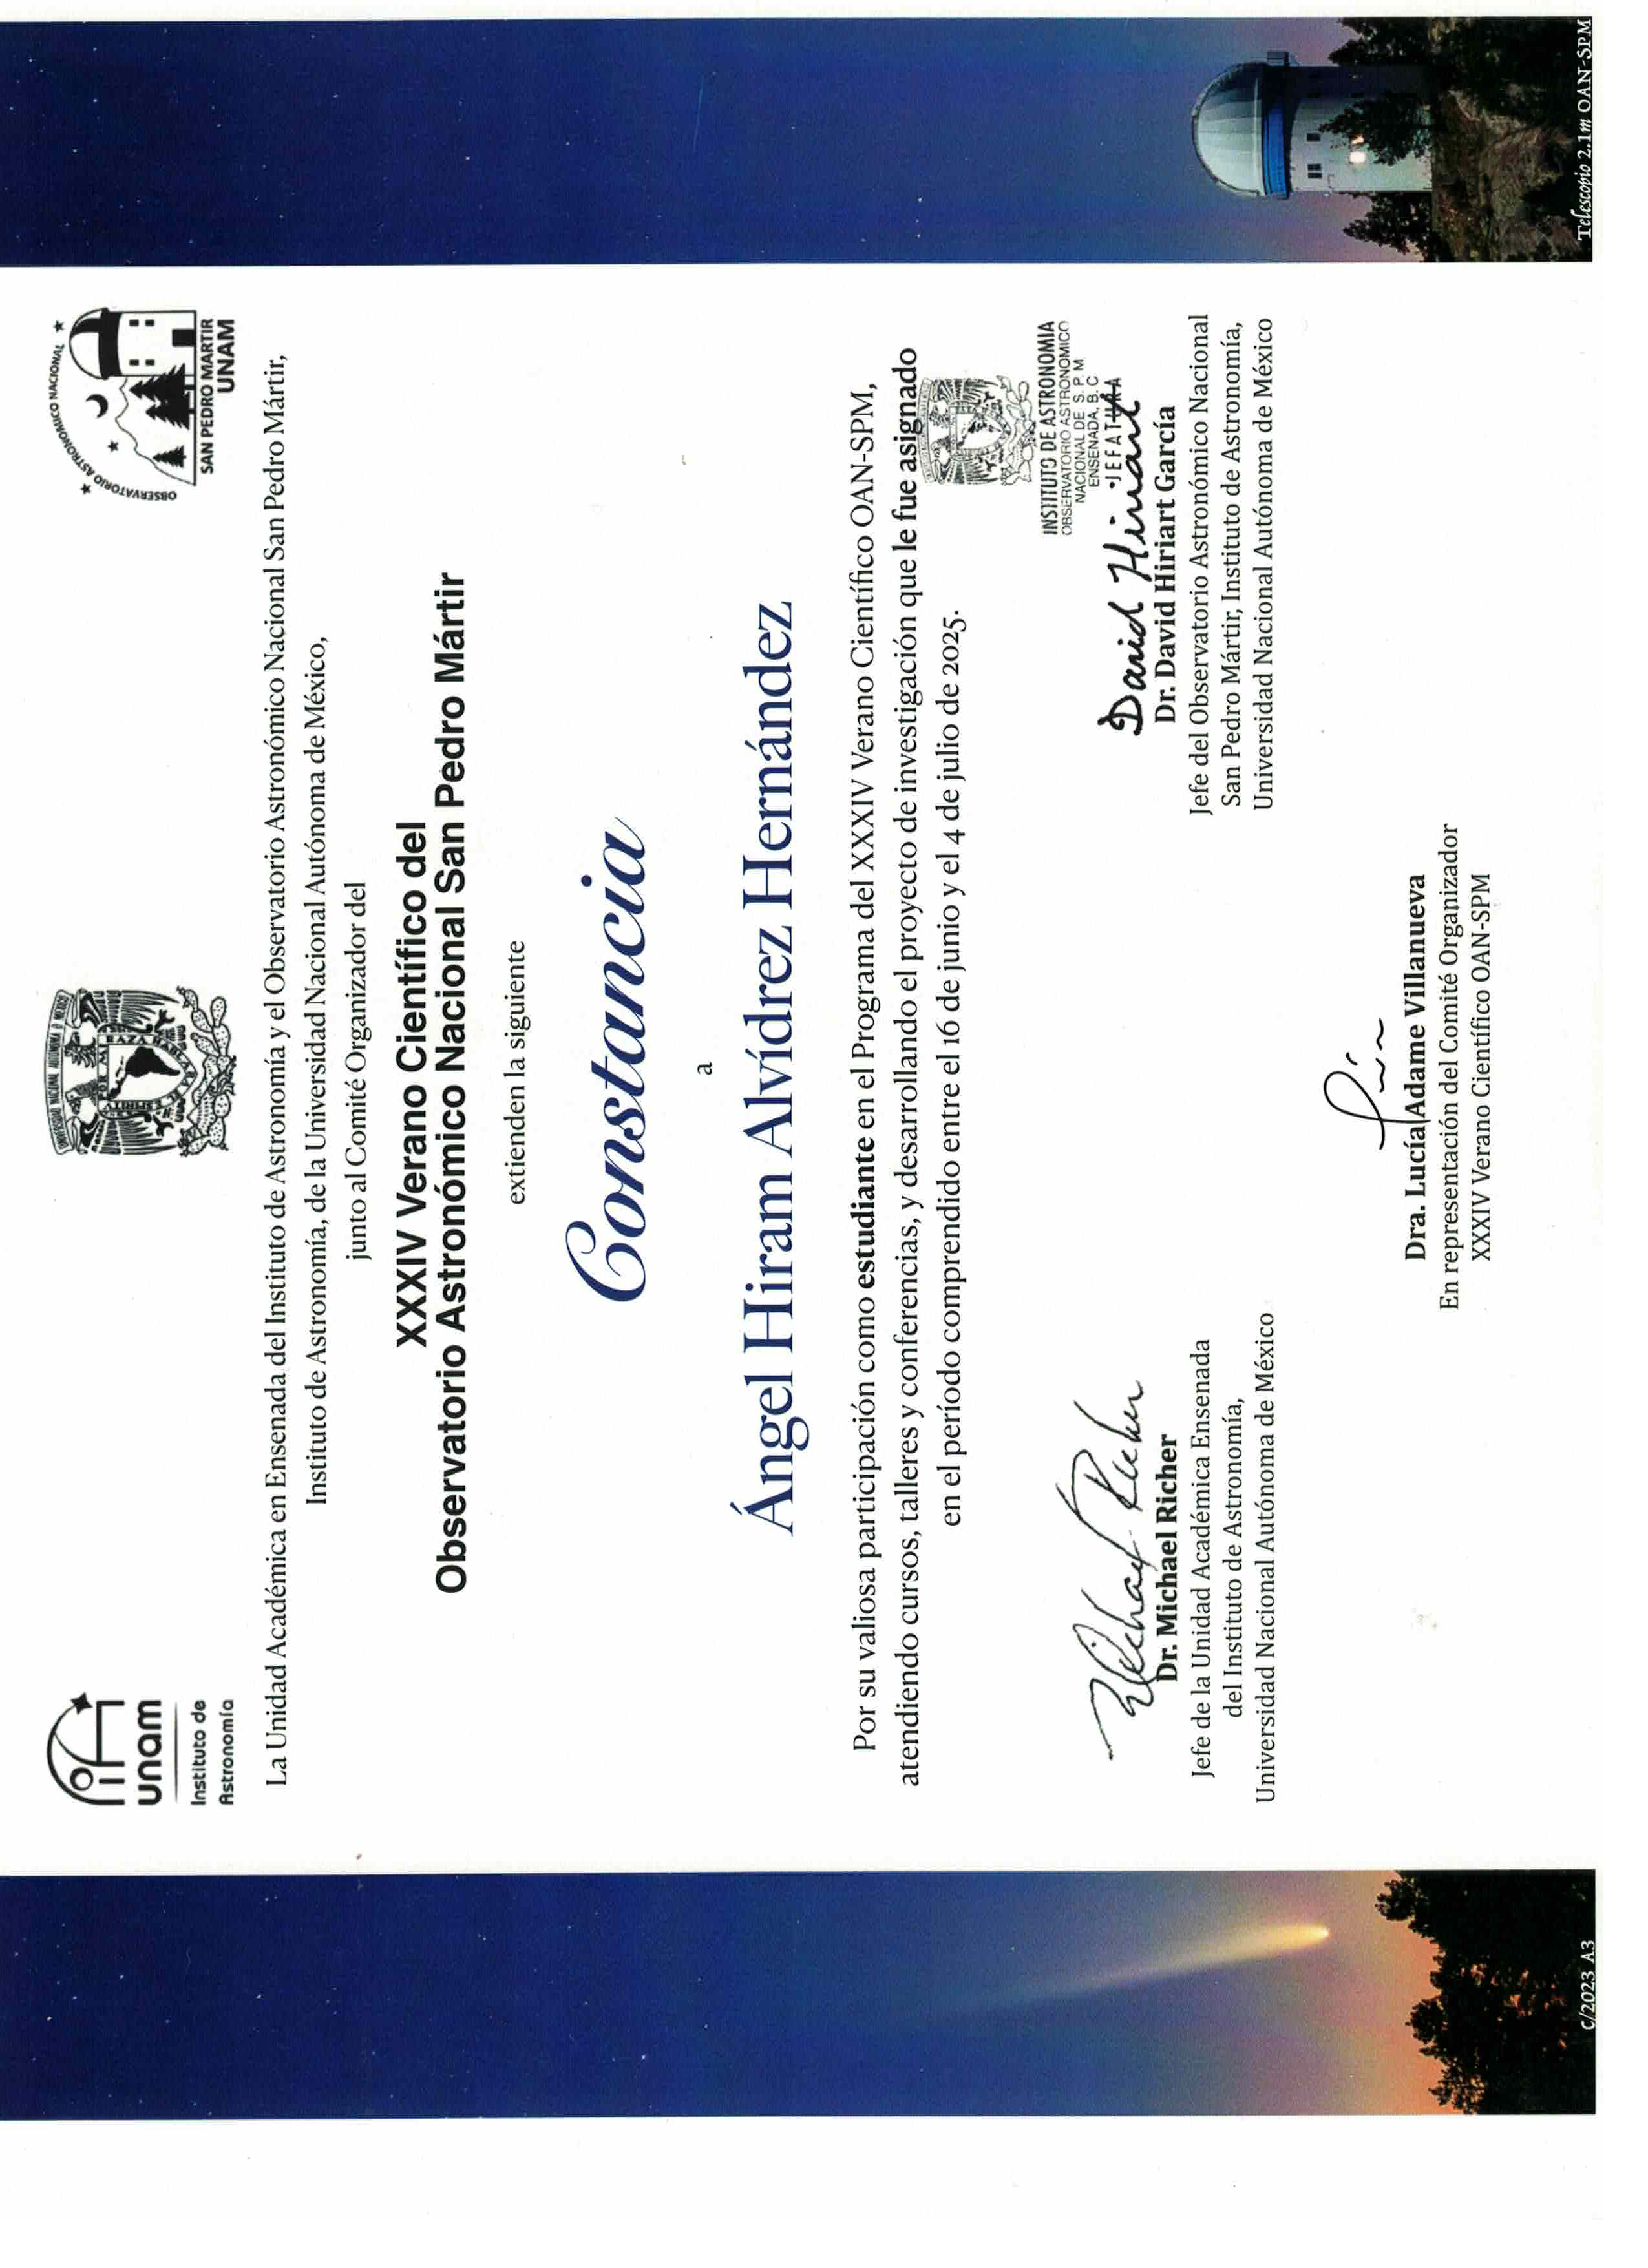
\includepdf[pages=-]{ConstanciaOAN.png}

\phantomsection
\addcontentsline{toc}{subsection}{Fundamentals of Semiconductors Certificate}

\includepdf[pages=-]{ConstanciaSemiconductores.png}

\phantomsection
\addcontentsline{toc}{subsection}{Integral Student Recognition}
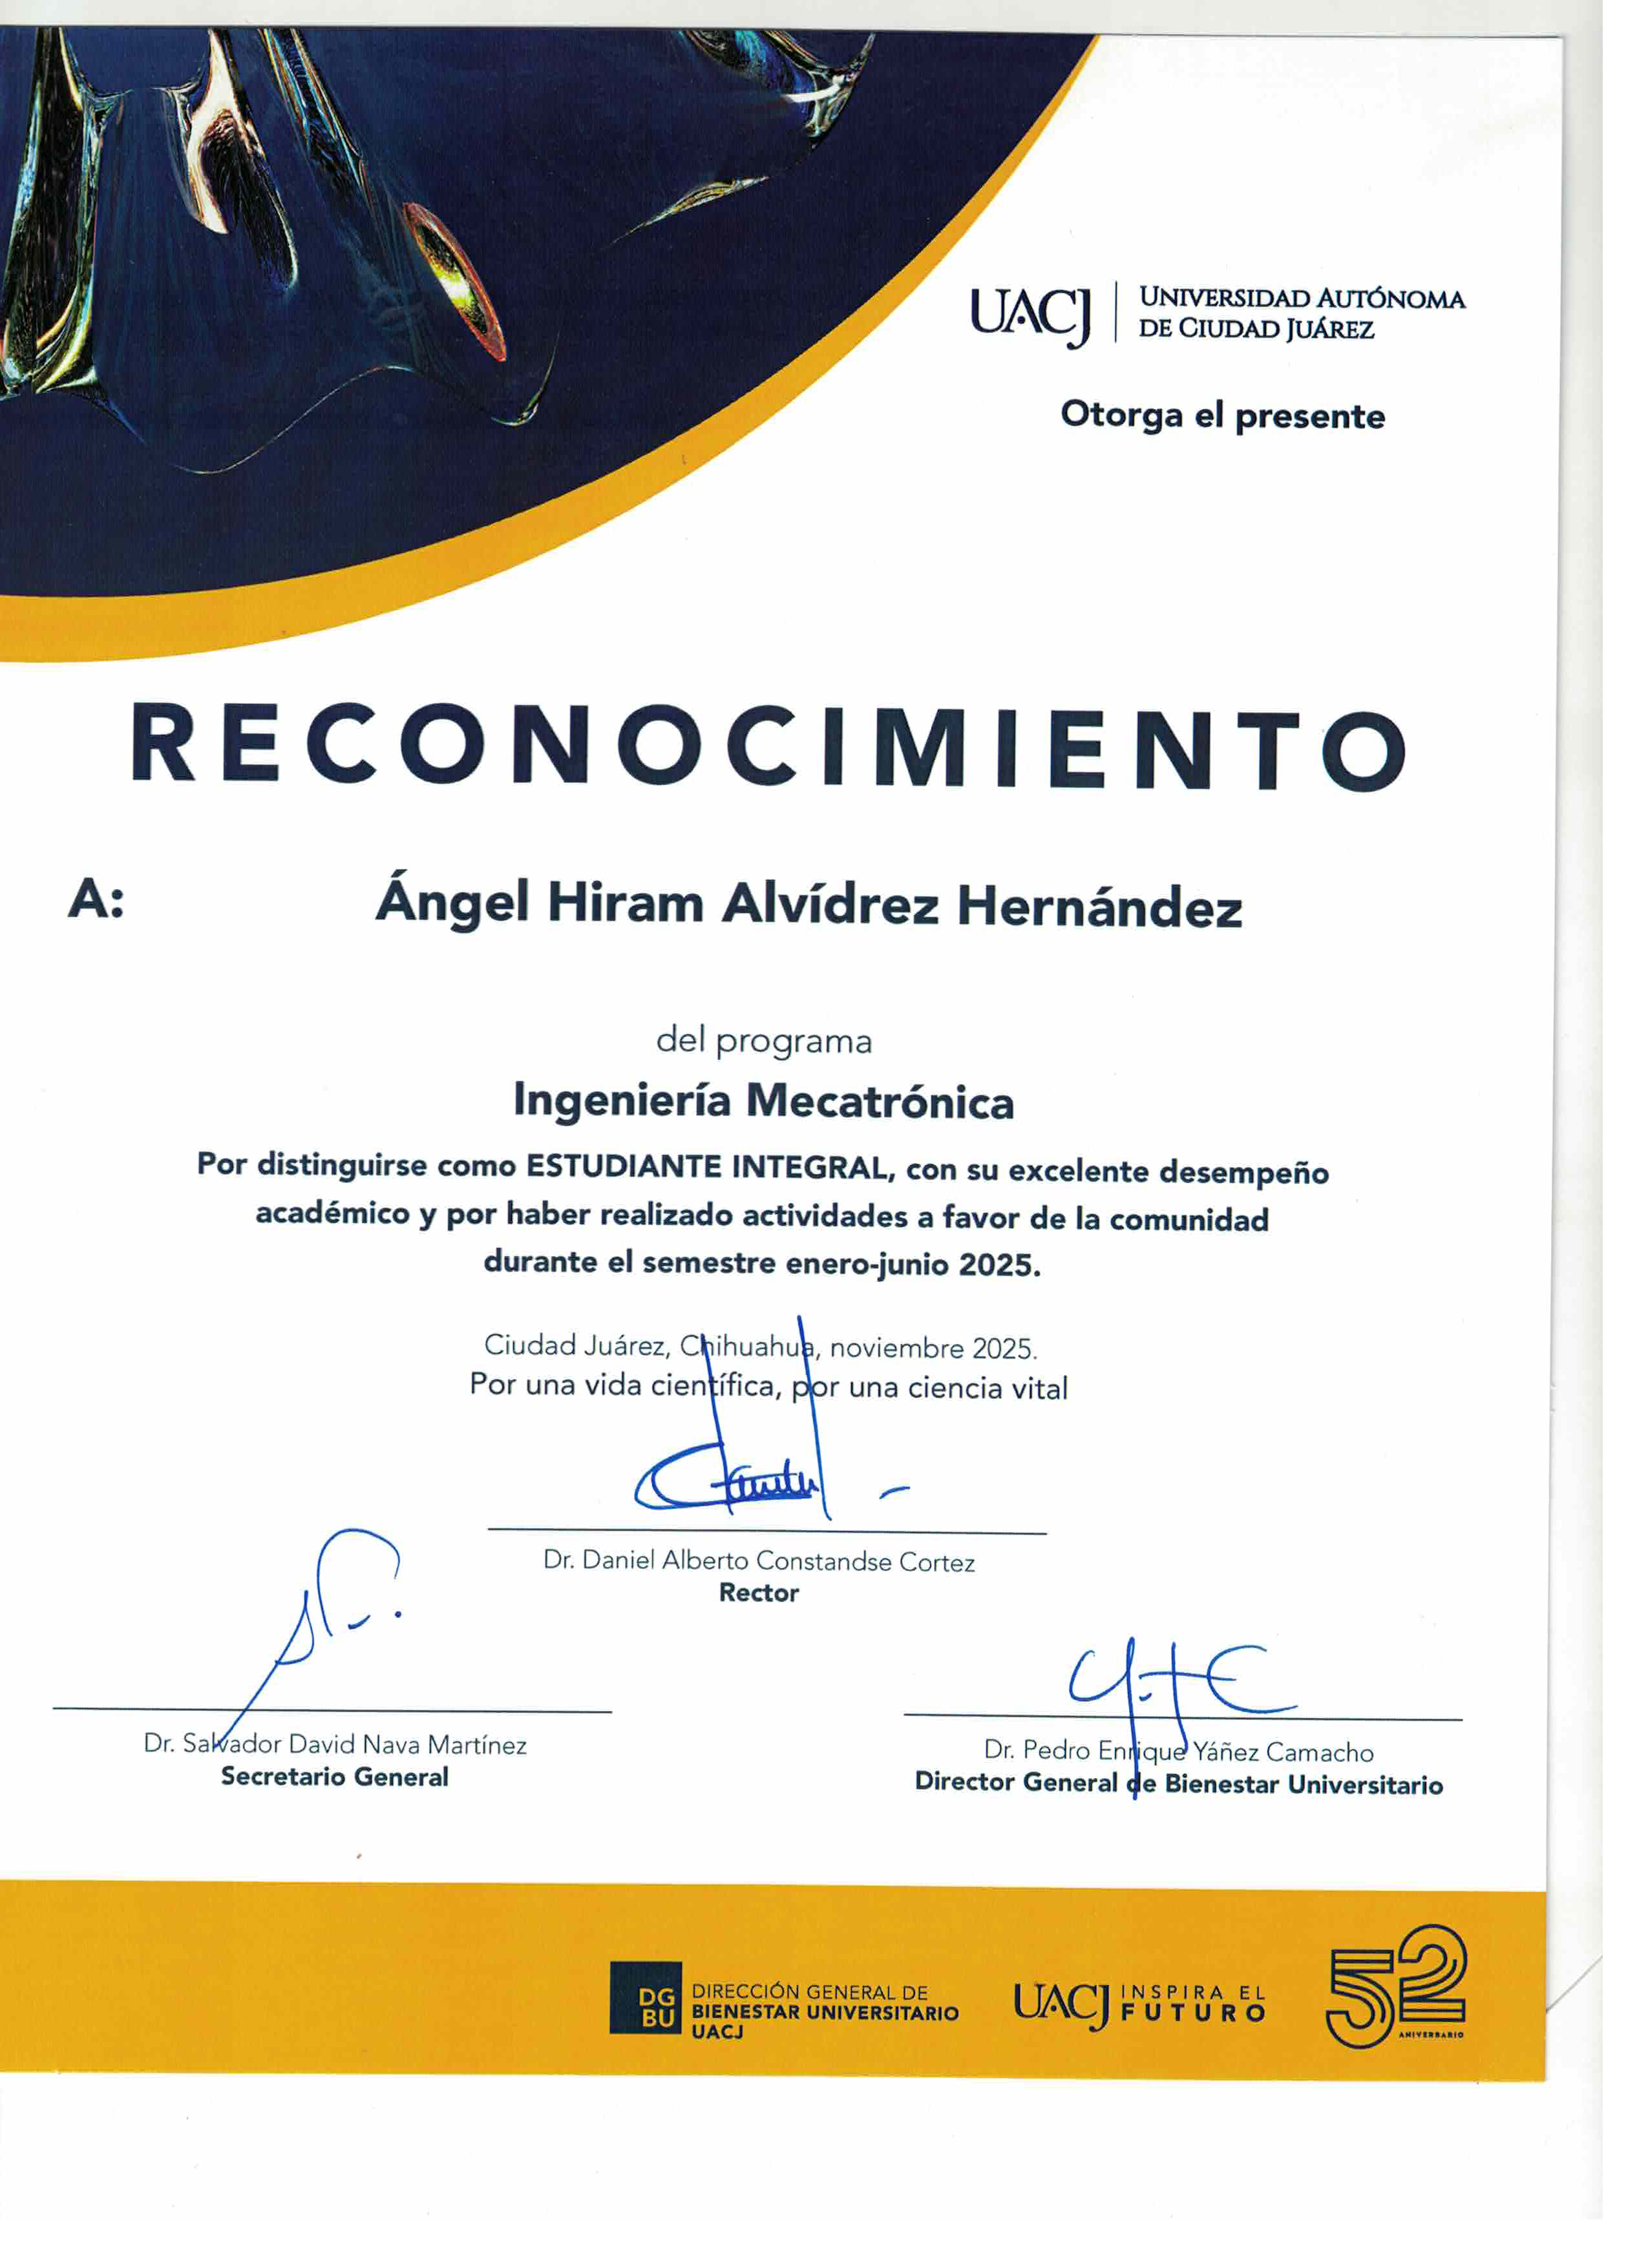
\includepdf[pages=-]{ReconocimientoEstudianteIntegral.png}

\phantomsection
\addcontentsline{toc}{subsection}{Recognition for Giving the Lecture: Are we really alone in the universe?}
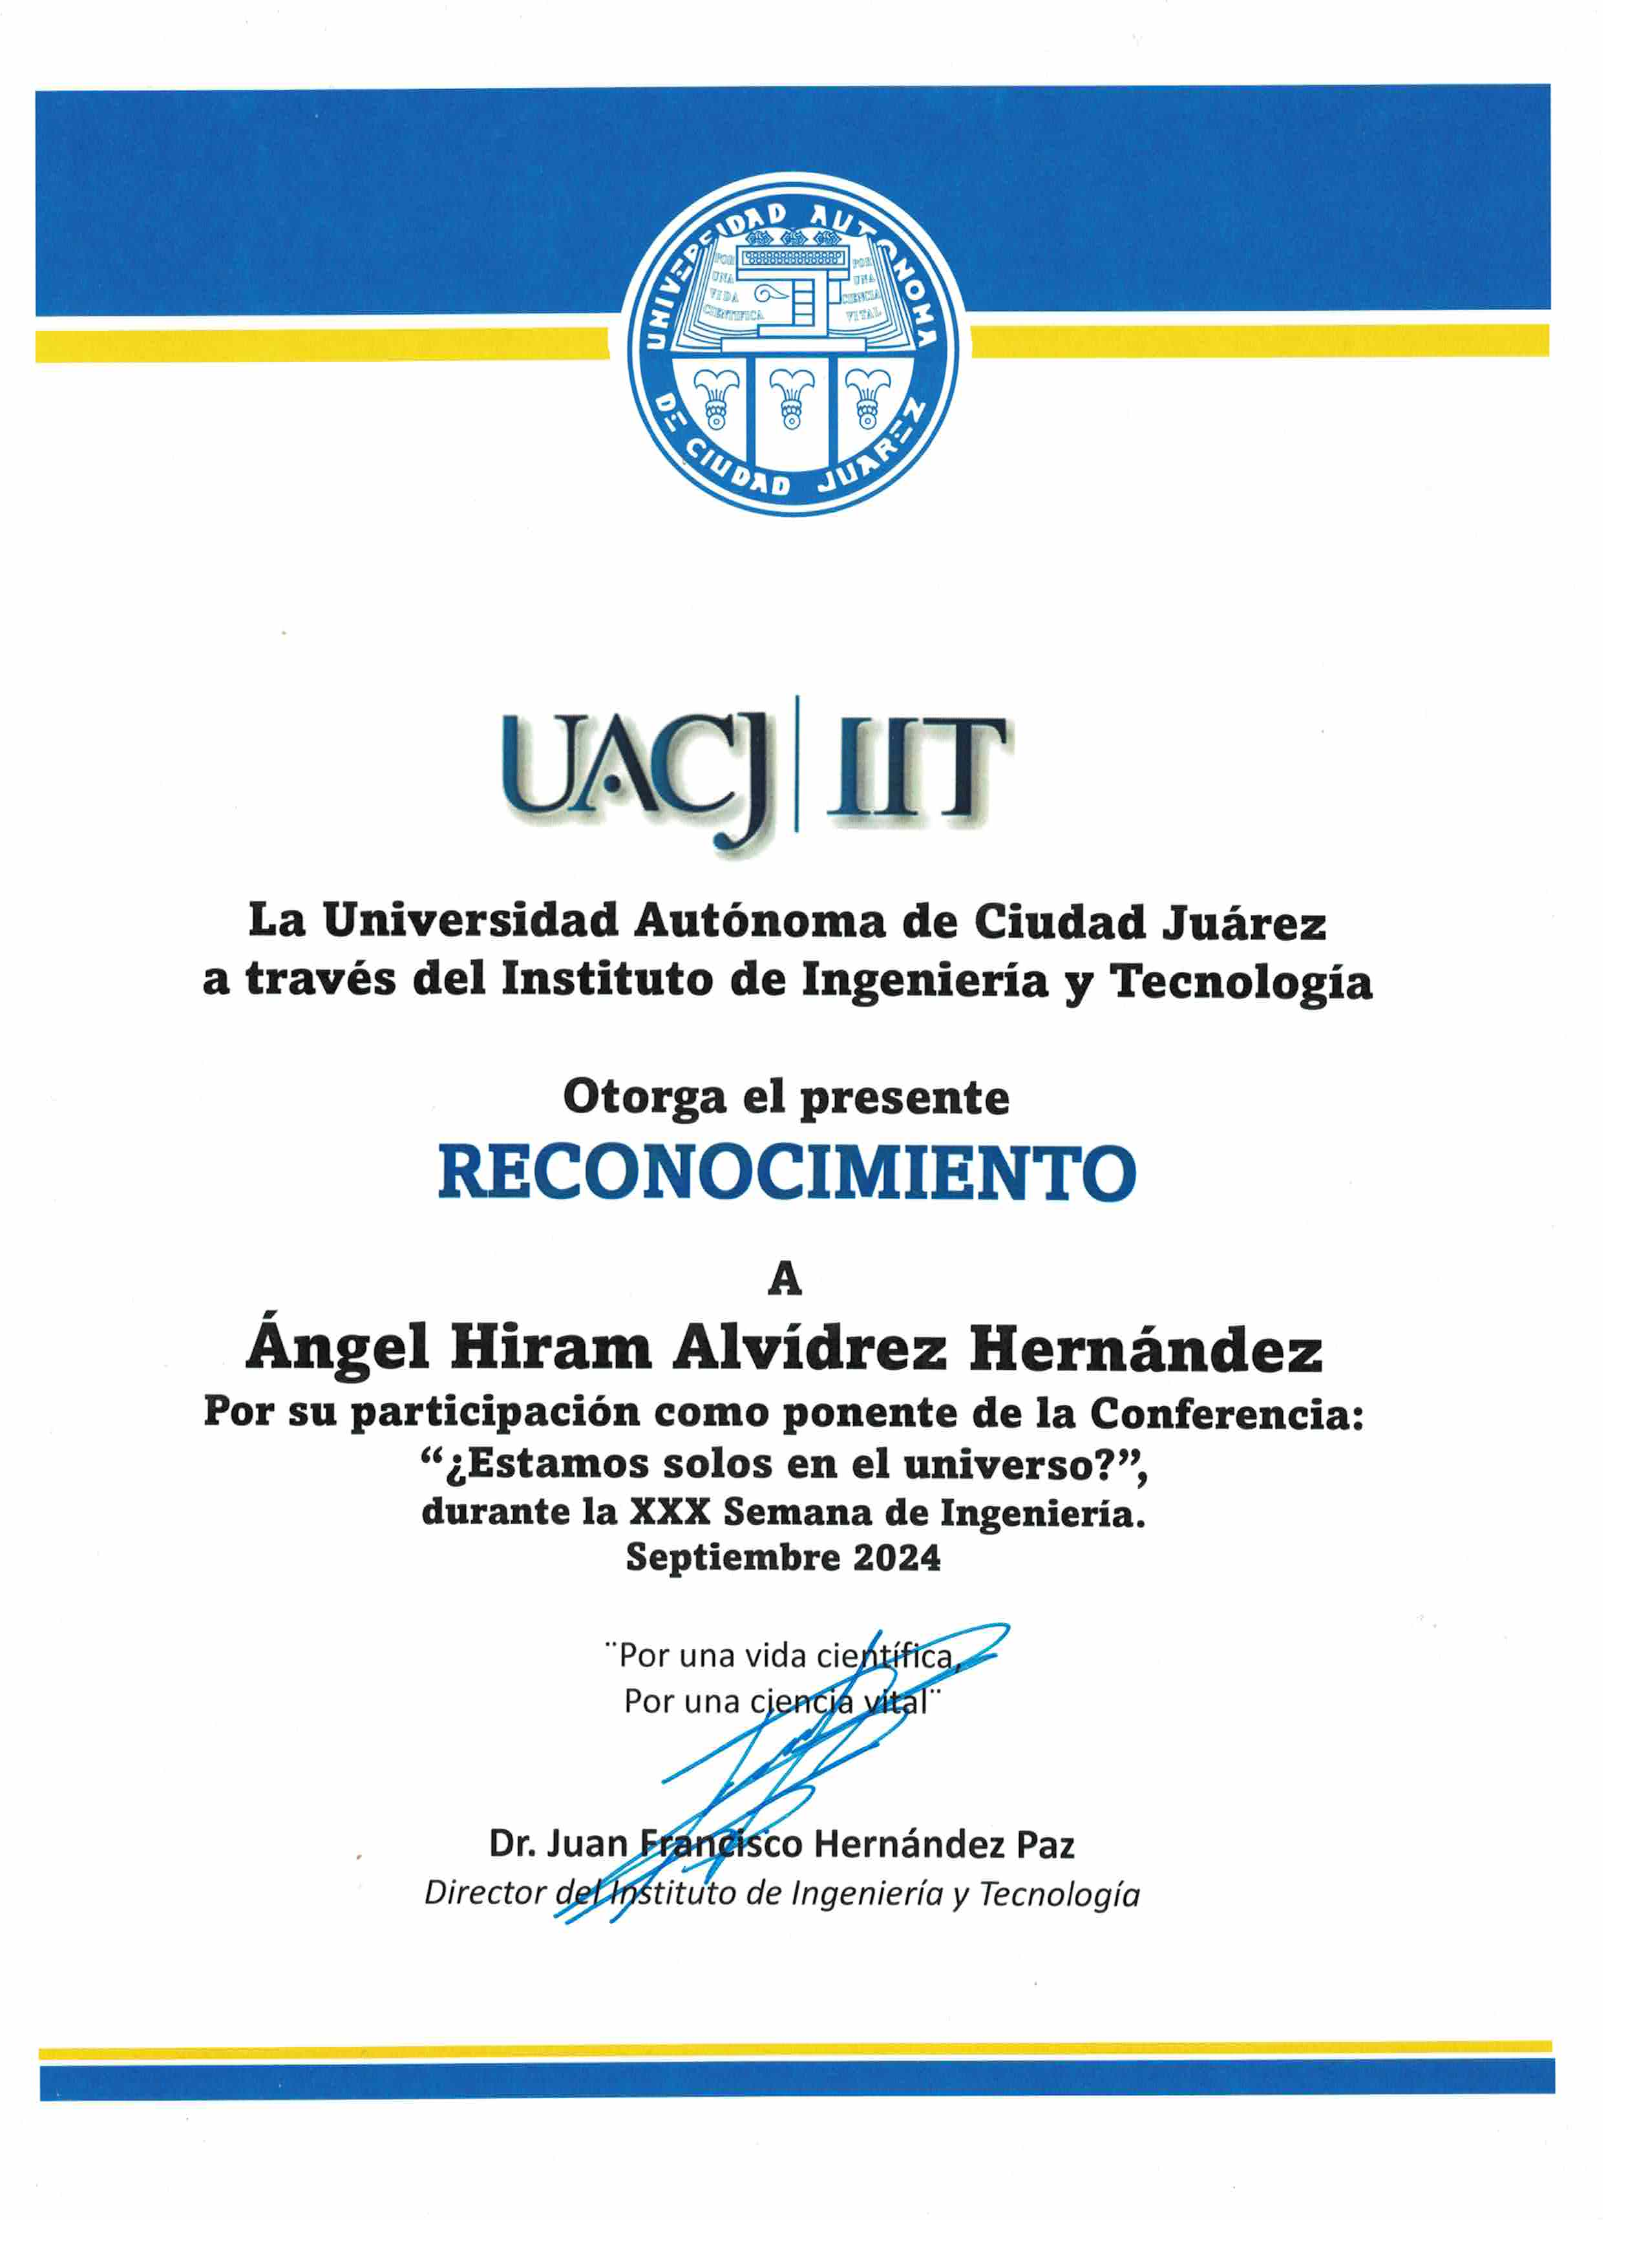
\includepdf[pages=-]{ReconocimientoConfSolosUniverso.png}

\phantomsection
\addcontentsline{toc}{subsection}{Recognition for Giving the Lecture: The deaths of the Universe}

\includepdf[pages=-]{ReconocimientoConfMuertesUniverso.png}

% ======= Engineering Projects and Practices =======
\phantomsection
\addcontentsline{toc}{section}{Engineering Projects and Practices}

\phantomsection
\addcontentsline{toc}{subsection}{Underactuated Biped Based on a 5-Bar Mechanism}
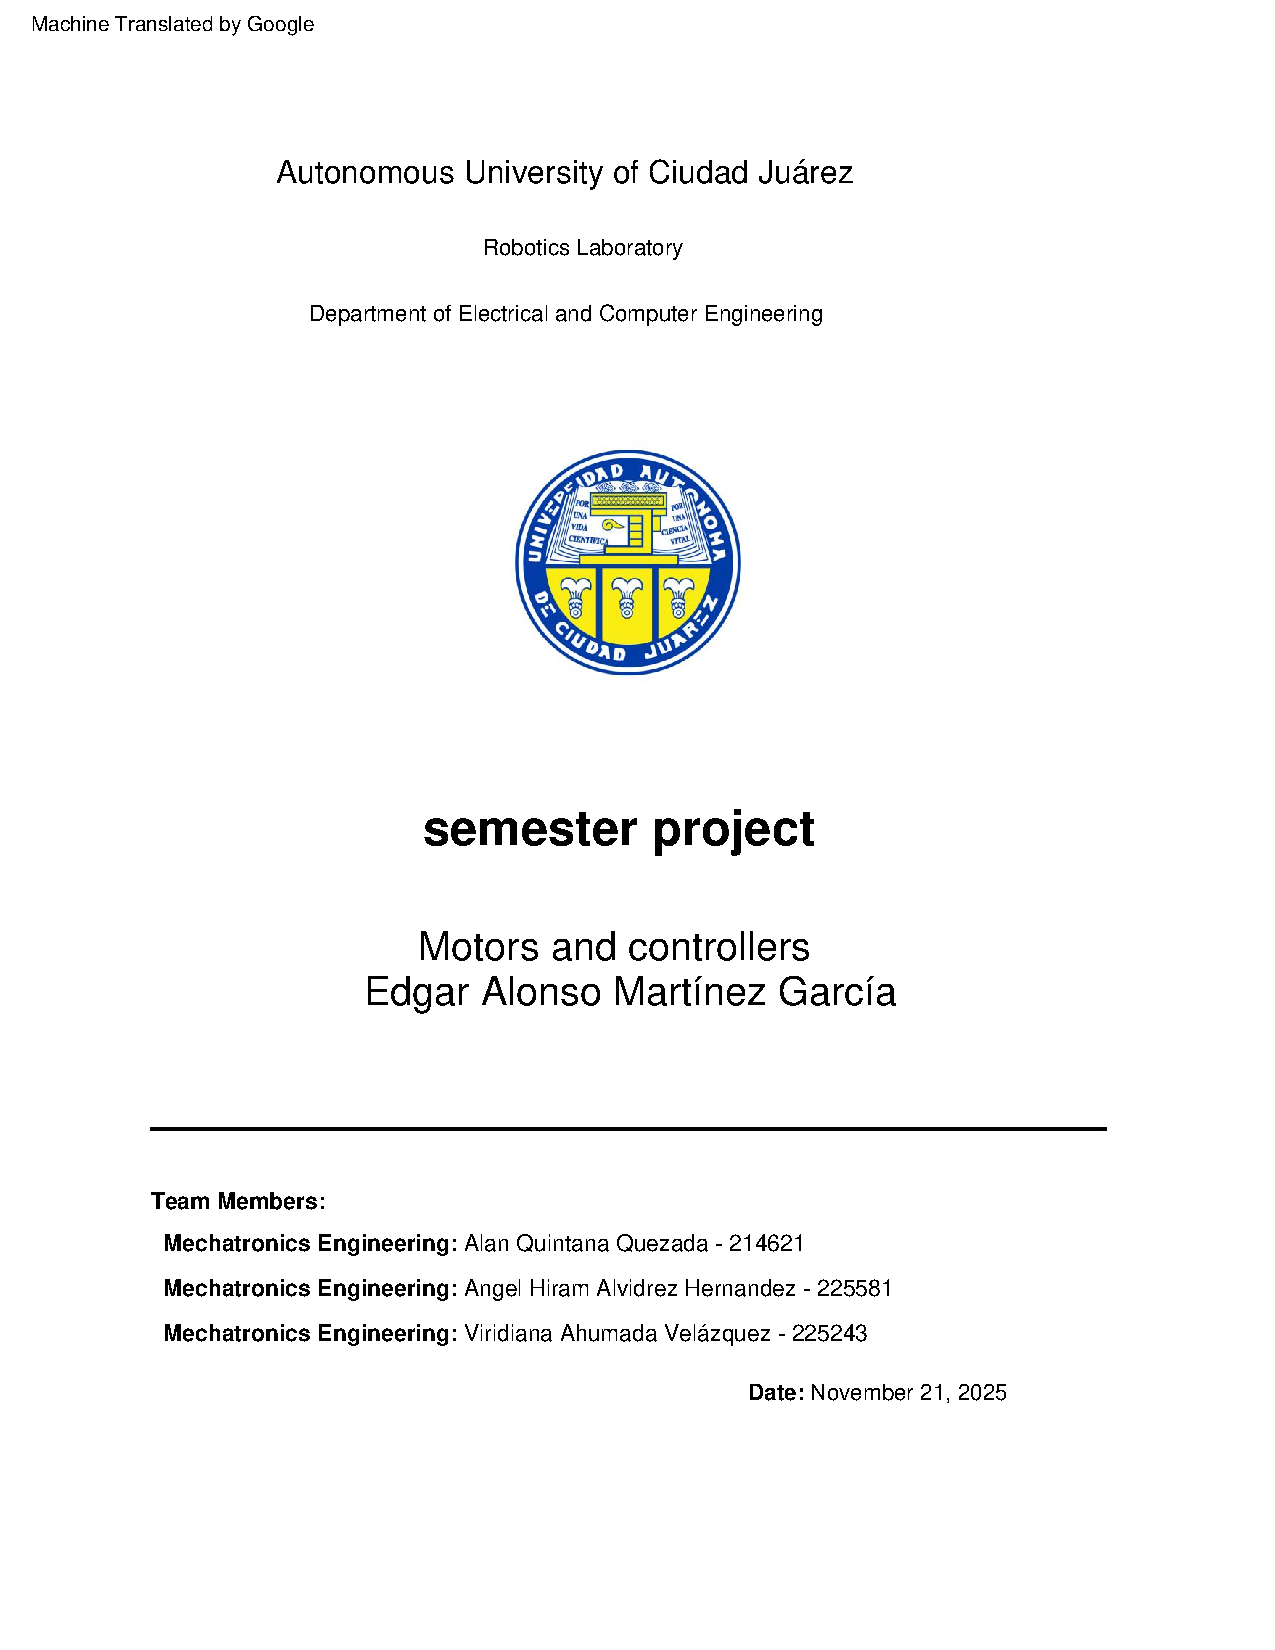
\includepdf[pages=-]{ProyectoSemestral_MotoresyControladores.pdf}

\phantomsection
\addcontentsline{toc}{subsection}{Telescope Control Electronics Upgrade}
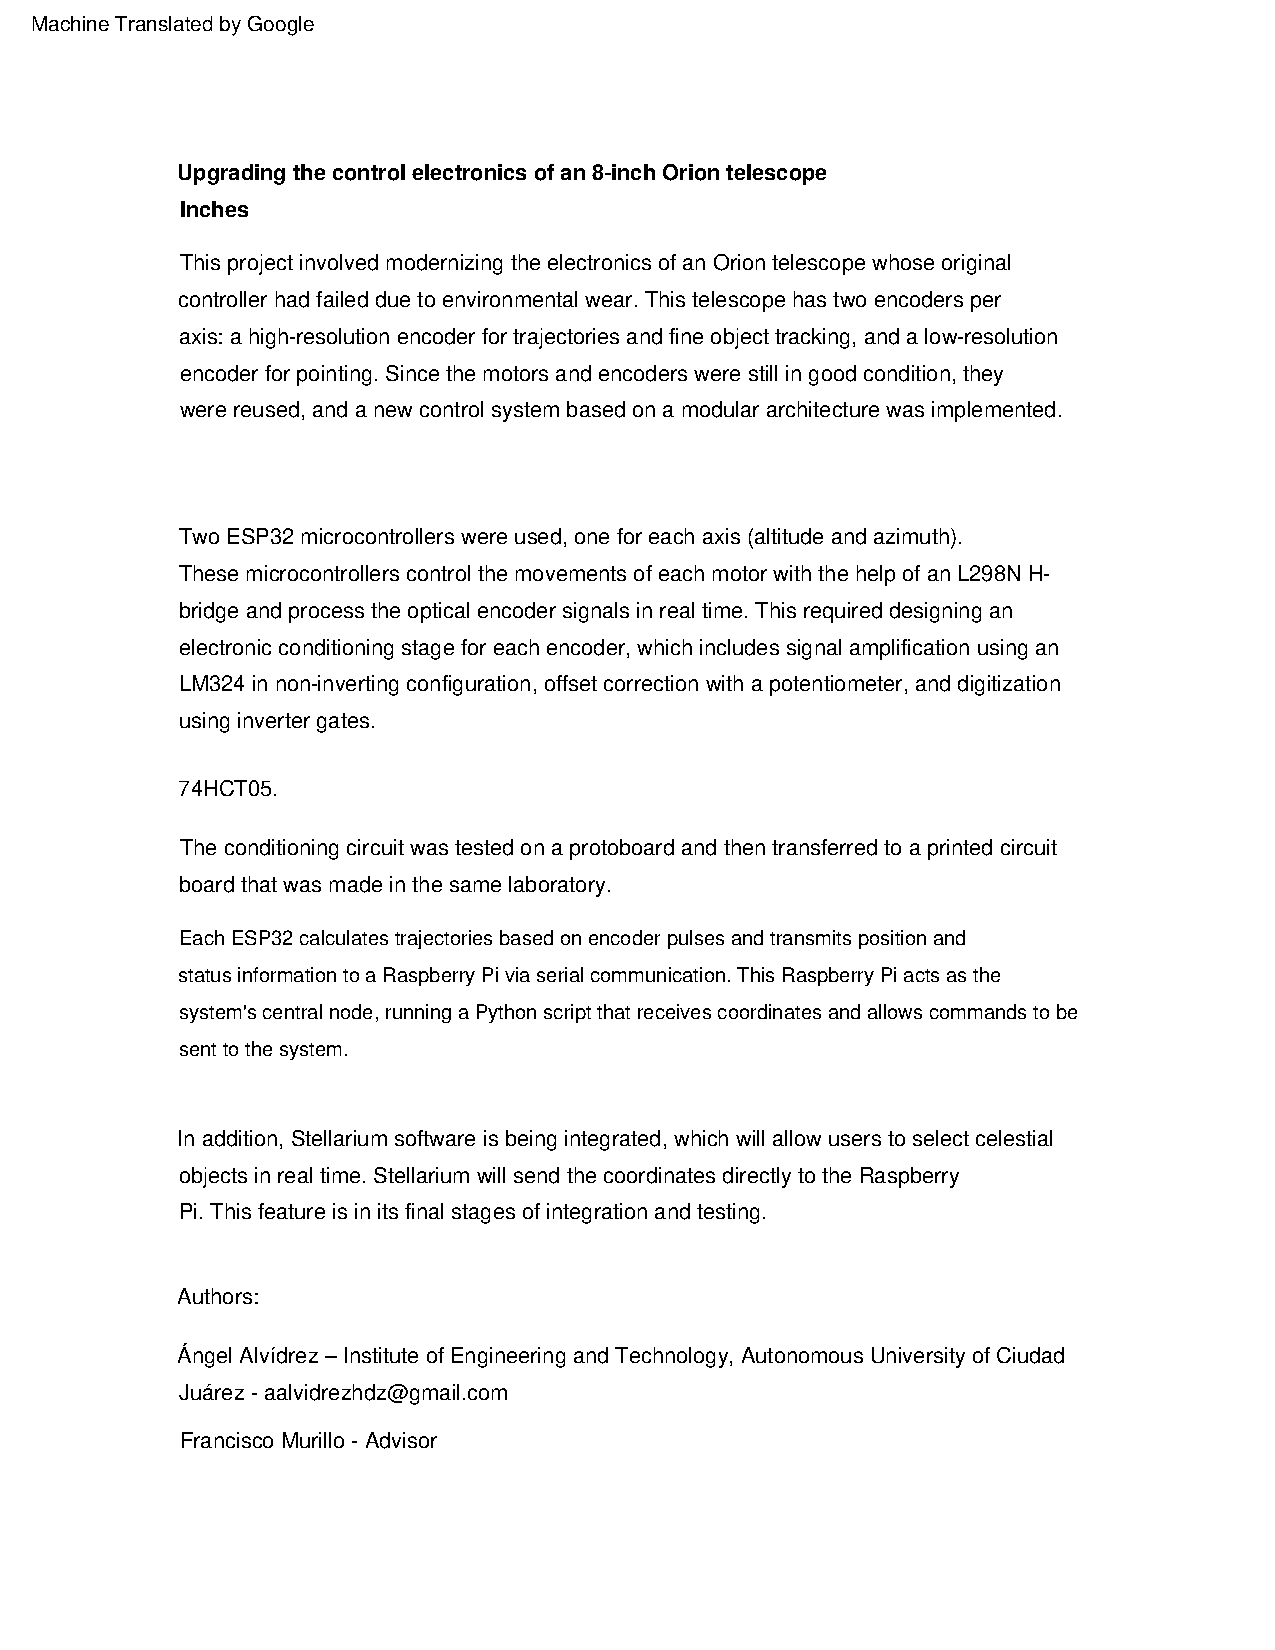
\includepdf[pages=-]{telescopio.pdf}

\phantomsection
\addcontentsline{toc}{subsection}{Transistor-Based Guitar Amplifier}
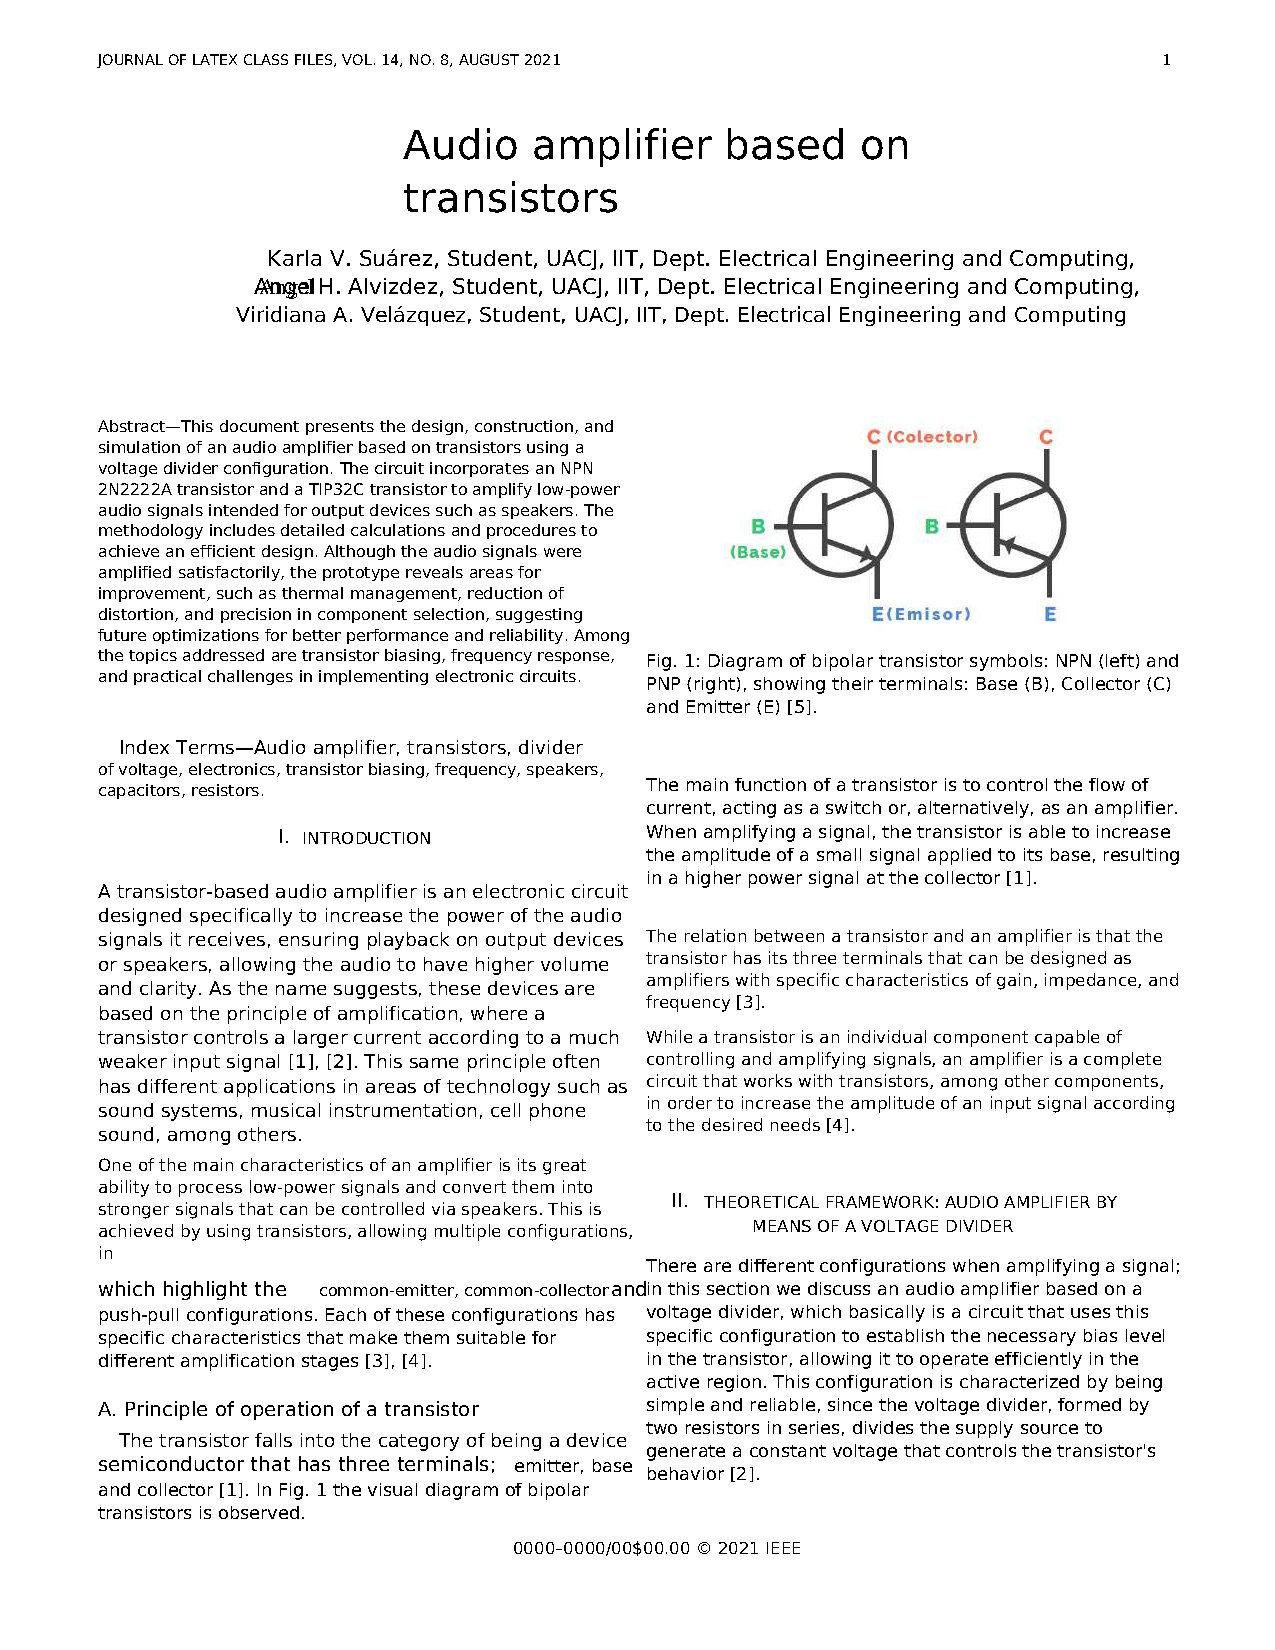
\includepdf[pages=-]{amplificador.pdf}

\phantomsection
\addcontentsline{toc}{subsection}{PID Position Control of a Cart}
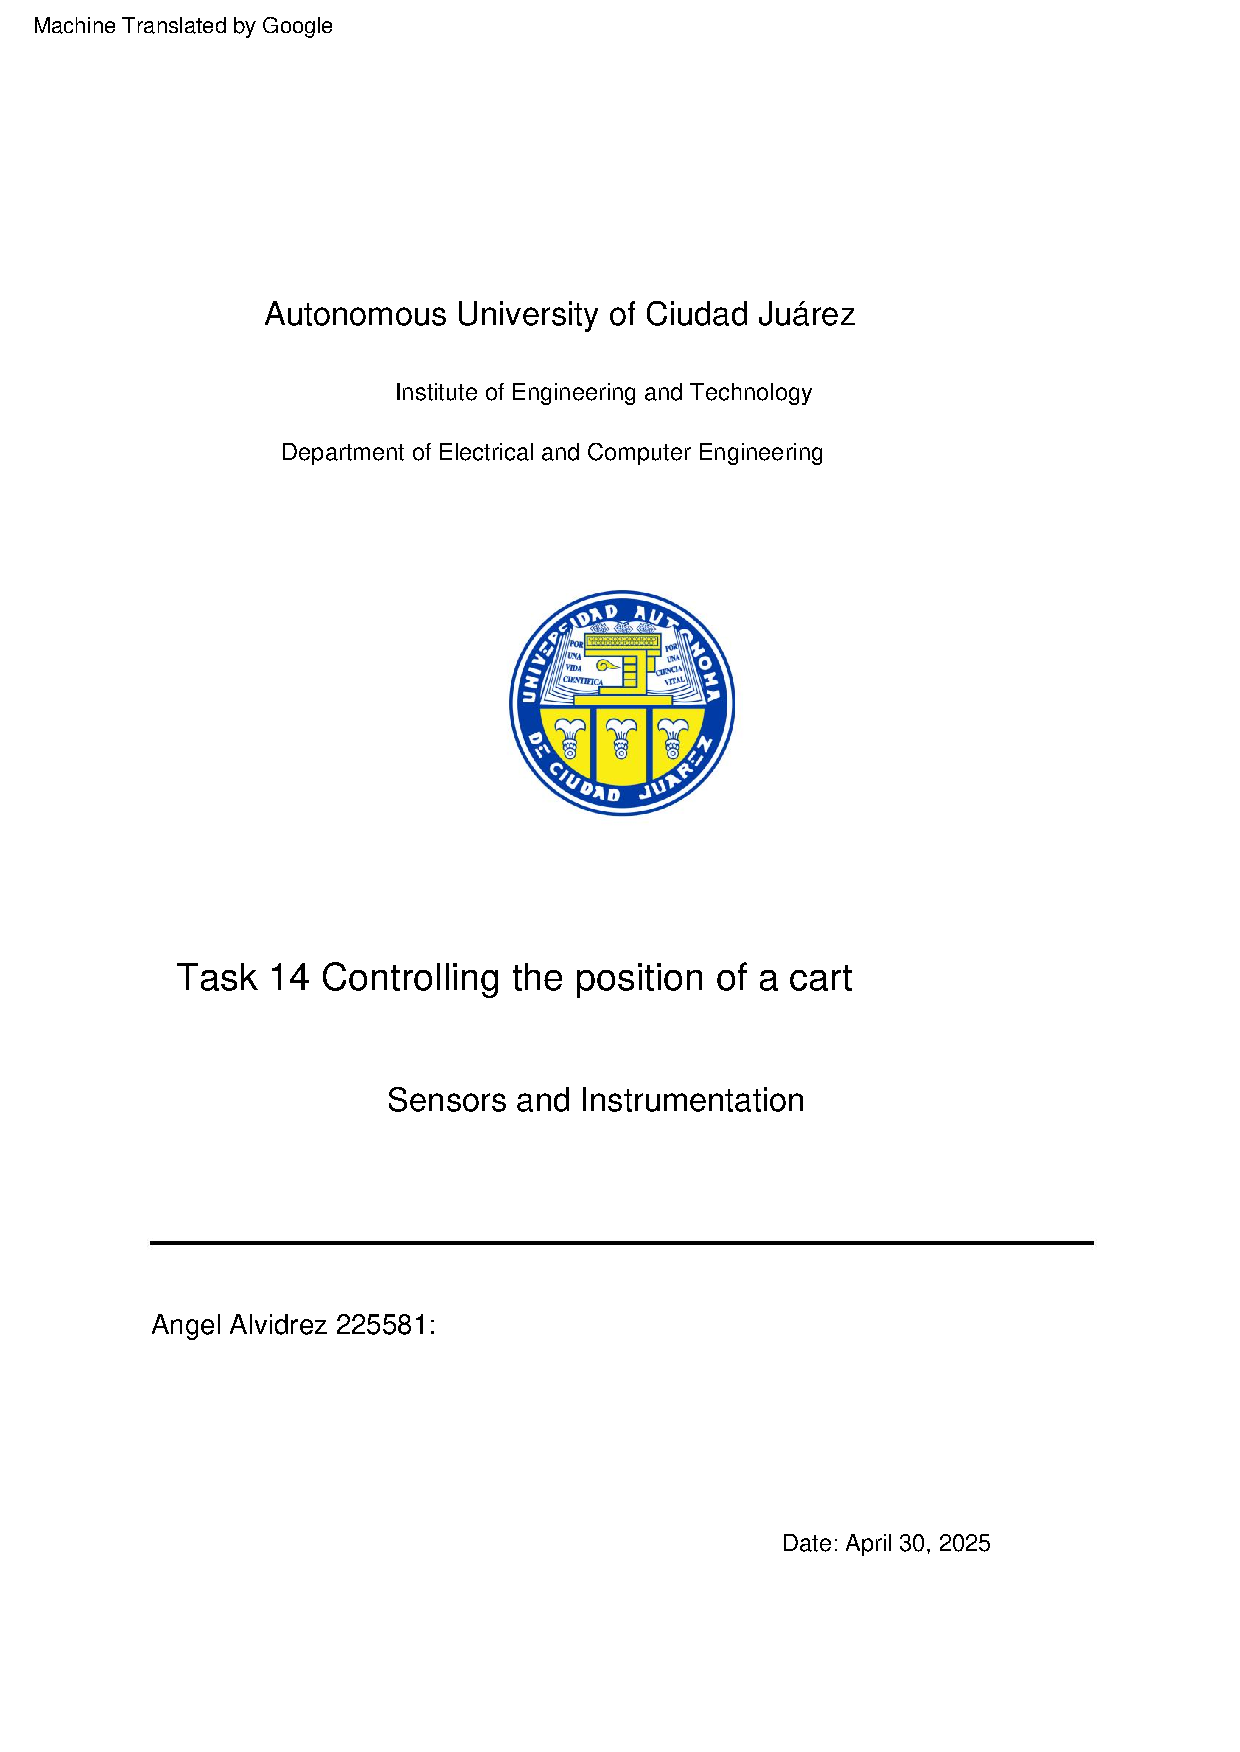
\includepdf[pages=-]{Control_de_Posicion_Carrito_PID.pdf}

\phantomsection
\addcontentsline{toc}{subsection}{Line Follower Cart}
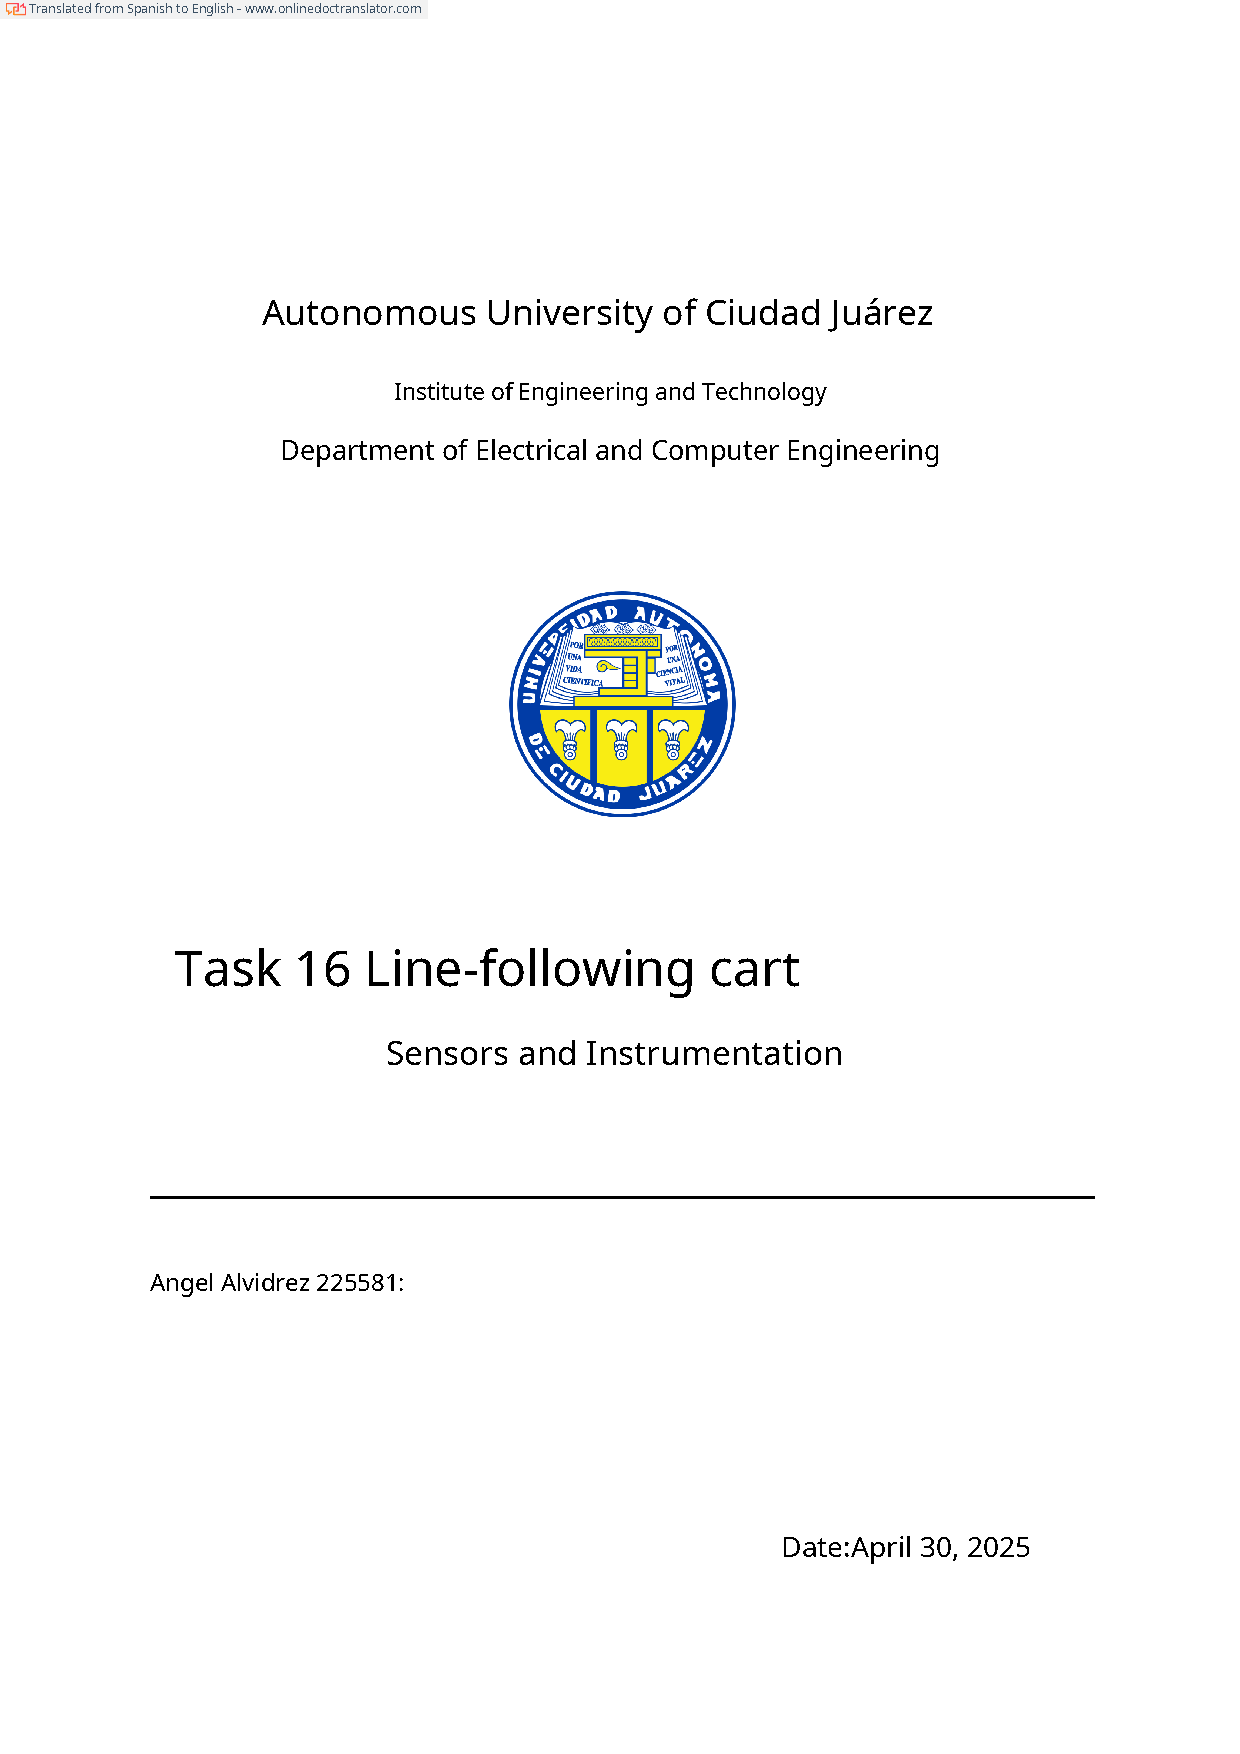
\includepdf[pages=-]{Carrito_Seugidor_de_lineas.pdf}

\phantomsection
\addcontentsline{toc}{subsection}{Clap-Activated Light Switch}
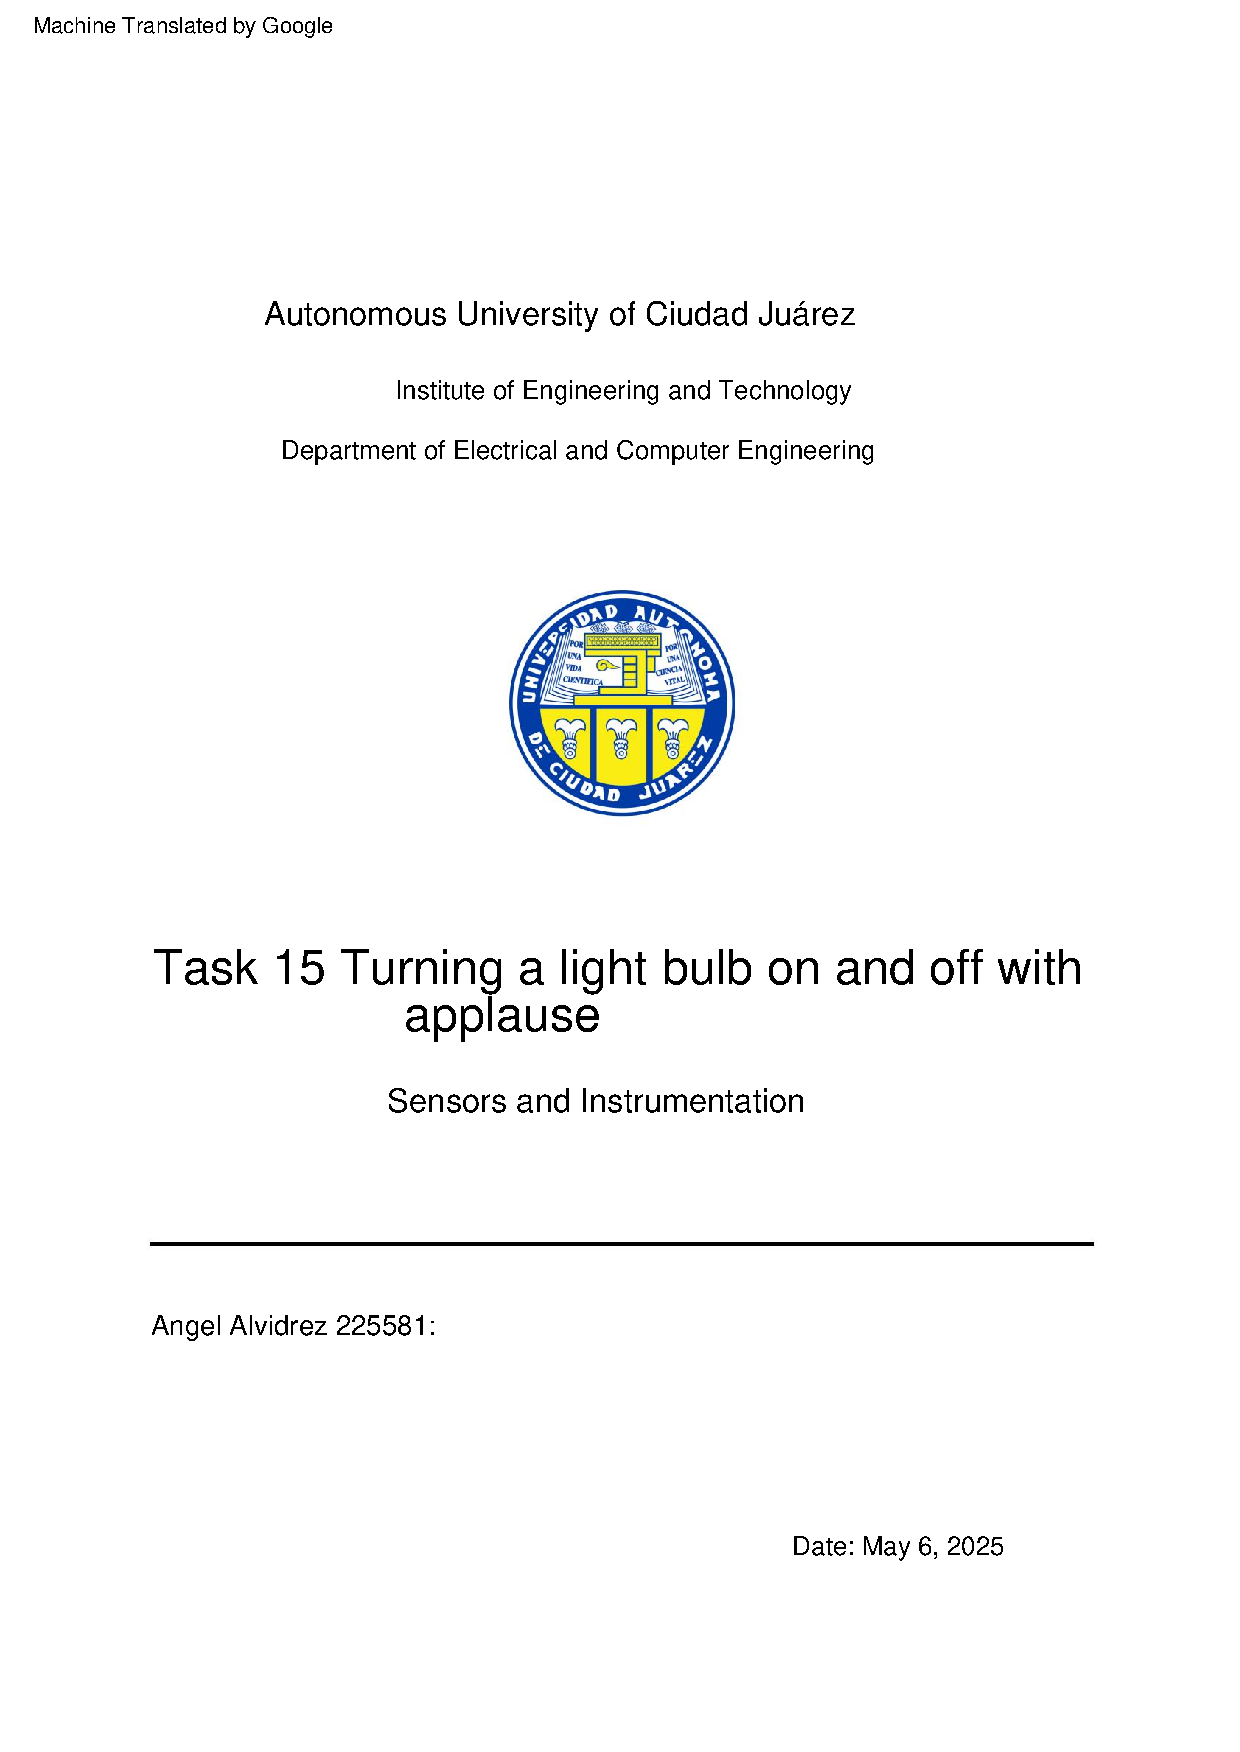
\includepdf[pages=-]{Sensor_De_Aplausos_Apagado_Prendido_Foco.pdf}

\phantomsection
\addcontentsline{toc}{subsection}{IoT Irrigation System (ESP32 + Blynk)}

\includepdf[pages=-]{Sistema_De_Riego_IOT.pdf}

% ======= Publications and Academic Works =======
\newpage
\phantomsection
\addcontentsline{toc}{section}{Publications and Academic Works}

\section*{Publications and Academic Works}

\phantomsection
\addcontentsline{toc}{subsection}{Article under review: Kinematic Modelling of Five-Bar Bipedal Locomotion}

\subsection*{Article under review: Kinematic Modelling of Five-Bar Bipedal Locomotion}

\textbf{Kinematic Modelling of Five-Bar Bipedal Locomotion: An Analytical Approach}

\vspace{0.3cm}

\textit{Status: Under Review}

\textit{Conference: 30th International Conference on Methods and Models in Automation and Robotics (MMAR 2026)}

\textit{Submission ID: 3077}

\vspace{0.3cm}

\textbf{Authors:} Ángel H. Alvídrez-Hernández, Edgar A. Martínez-García

\vspace{0.5cm}

\textbf{Description:}

This work presents an analytical model for the kinematics of a bipedal robot based on a five-bar mechanism. Direct and inverse kinematics equations are developed, as well as a deterministic mapping between the joint space and the task space. Furthermore, a Kalman filter is implemented for system state estimation, allowing for trajectory tracking and motion stabilization in an experimental prototype.

\vspace{0.7cm}

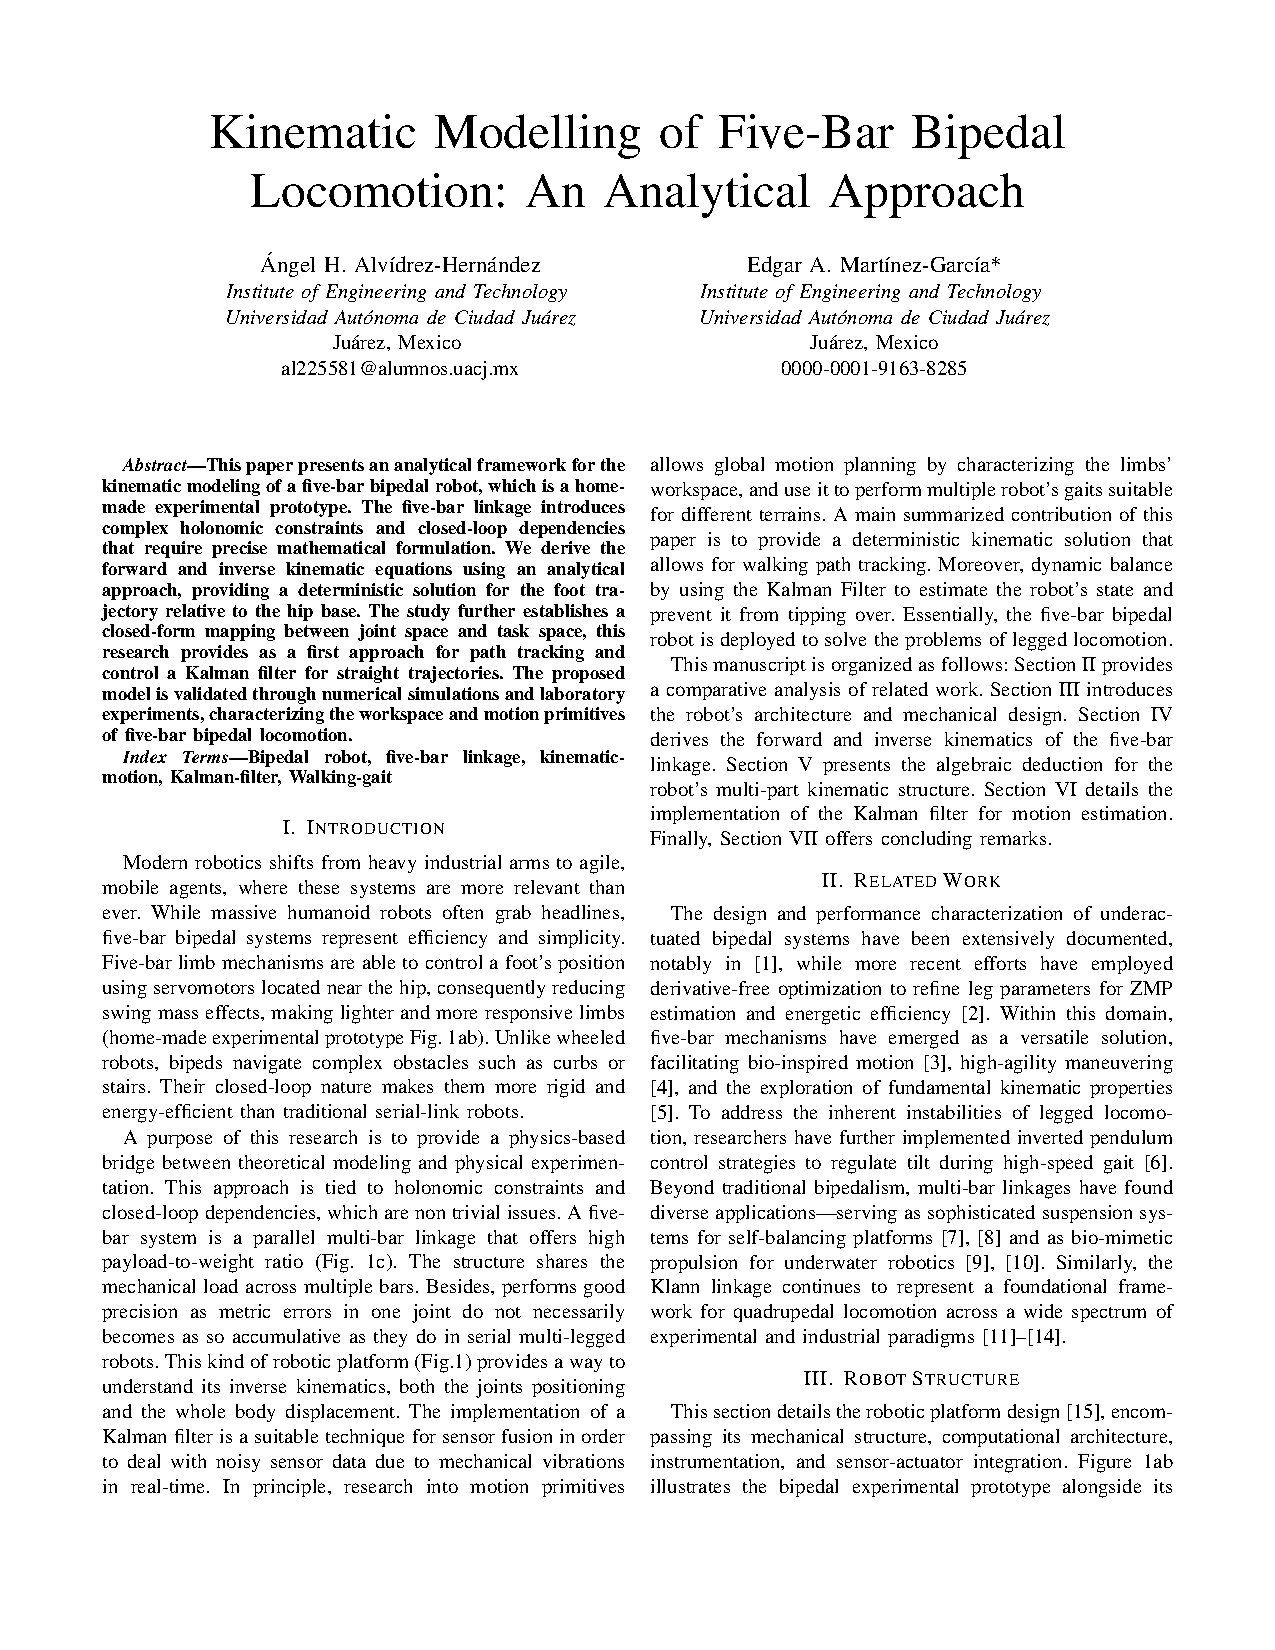
\includepdf[pages=-]{MMAR26_confBiped5b.pdf}